%!TEX root = ../main.tex

\section{Постановка задачи}

\begin{frame}{Физика процесса}
\begin{block}{Электрический пробой}
    Явление резкого возрастания тока в диэлектрике при приложении электрического напряжения выше критического.
\end{block}
\begin{itemize}
    \item Может возникать в стационарных/переменных/импульсных полях
    \item В ряде случаев связан с образованием тонкого проводящего канала
    \item Может приводить к развитию необратимых повреждений в материале
    \item В твердых телах -- наиболее сложный комплекс механизмов, богатая физика
\end{itemize}
\end{frame}


\begin{frame}{Математическая модель}
\begin{block}{Модель типа диффузной границы}
    Вещество находится в разных фазах. Состояние вещества описывается гладкой функцией $\phi(\vx, t)$ -- фазовым полем.
\end{block}
\begin{itemize}
    \item Фазы: $\phi = 1$ -- неповрежденная среда, $\phi = 0$ -- полностью разрушенная
    \item Зона $\phi \in (0, 1)$ -- диффузная граница
    \item На разрушение среды тратится энергия
    \item Возможно учесть произвольную геометрию раздела фаз
\end{itemize}
\begin{figure}
    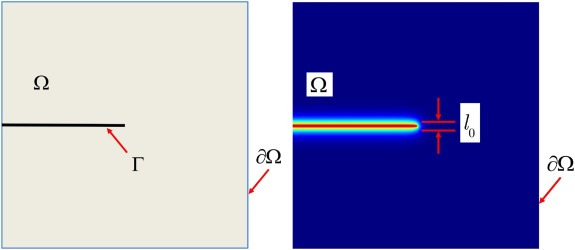
\includegraphics[width=0.5\textwidth]{figures/diffuse_edge.jpg}
\end{figure}
\end{frame}


\begin{frame}{Математическая модель}
%\vspace{-0.3cm}
\begin{block}{Уравнения динамики системы}
    \vspace{-2mm}
    \begin{gather*}
        \Div(\epsilon[\phi] \nabla \Phi) = -\rho_E \\
        \partt{\rho_E} = \Div(\sigma[\phi] \nabla \Phi) \\
        \cfrac{1}{m} \partt{\phi} = -F'_\phi( \phi; \| \nabla \Phi \|) + \cfrac{\Gamma}{2} \Delta \phi + \beta \Gamma l^2 \Div \left( \| \nabla \phi \|_2^2 \nabla \phi \right)
    \end{gather*}
    \vspace{-4mm}
\end{block}
\begin{itemize}
    \item $m$, $\Gamma$, $l$, $\beta$ -- параметры модели, константы
    \item $F(\phi; \| \nabla \Phi \|)$ -- определенная нелинейная функция
\end{itemize}
\end{frame}


\begin{frame}{Математическая модель}
\vspace{-3mm}
\begin{gather*}
    F(\phi; \| \nabla \Phi \|) = -\half \epsilon[\phi] \cdot \| \nabla \Phi \|_2^2 + \cfrac{\Gamma}{l^2} [1 - f(\phi)] \\
    \begin{alignedat}{3}
        \epsilon[\phi] &= \epsilon(\vx, t) &&= \cfrac{\epsilon_0(\vx)}{f[\phi(\vx, t)] + \delta_\epsilon} \\
        \sigma[\phi] &= \sigma(\vx, t) &&= \cfrac{\sigma_0(\vx)}{f[\phi(\vx, t)] + \delta_\sigma}
    \end{alignedat} \\[2mm]
    f(\phi) = 4 \phi^3 - 3 \phi^4
\end{gather*}
\vspace{-6mm}
\begin{itemize}
    \item $\delta_\epsilon$, $\delta_\sigma$ -- регуляризующие параметры
    \item $f(\phi)$ -- интерполирующая функция
\end{itemize}
\vspace{1mm}
\parind Модель описана в \cite{zipunova_computational} на основе \cite{pitike_dielectric_breakdown}
\end{frame}


{\nologo
\begin{frame}{Функционалы энергии}
\vspace{-5mm}
\begin{itemize}
    \item Плотность энергии электрического поля:
    \[
        w_{E} = \half \epsilon[\phi] \cdot \| \nabla \Phi \|_2^2.
    \]
    \item Плотность энергии, отнесенной к каналу пробоя:
    \[
        w_\text{br} = %
        \color{light_grey}\left[\color{black} \cfrac{\Gamma}{l^2} [1 - f(\phi)] \color{light_grey}\right]\color{black} + %
        \color{light_grey}\left[\color{black} \cfrac{\Gamma}{4} \| \nabla \phi \|_2^2 + \cfrac{\beta}{4} \Gamma l^2 \| \nabla \phi \|_2^4 \color{light_grey}\right]\color{black}.
    \]
\end{itemize}
\begin{columns}
\column{0.49\textwidth}
    \centering
    Свободная энергия Гельмгольца
    \[
        \psi = -w_E + w_\text{br}, \quad \Psi = \int\limits_\Omega \psi d \vx
    \]
\column{0.01\textwidth}
    \rule{0.4pt}{0.25\textheight}
\column{0.49\textwidth}
    \centering
    Внутренняя энергия
    \[
        w = w_E + w_\text{br}, \quad W = \int\limits_\Omega w d \vx
    \]
\end{columns}
\end{frame}
}